\PassOptionsToPackage{demo}{graphicx}
\documentclass[tikz, border=10mm]{standalone}
\usepackage[francais]{babel}
\usepackage[utf8]{inputenc}
\usepackage[T1]{fontenc}
\usetikzlibrary{positioning,calc,arrows.meta}
\begin{document}
  \begin{tikzpicture}
    [
      my text/.style={rounded corners=2pt, text width=50mm, font=\sffamily, draw=blue!20!black!50, line width=.5pt, align=left},
      my arrow/.style={rounded corners=2pt, draw=blue!20!cyan, line width=2.5mm, -{Triangle[]}},
    ]

    \node (b1) [my text] {1938: naissance de la société SNCASE (Société nationale de construction aéronautique du sud-est).};
    \node (b2) [right=5mm of b1, my text] {1943: le premier appareil à voilure tournante voit le jour à Marignane.\\1956: la SNCASE se transforme en SUD-EST-AVIATION.};
    \node (b3) [right=5mm of b2, my text] {1957: SUD-EST-AVIATION se transforme en SUD-AVIATION};

    \node (a2) [above=5mm of b2] {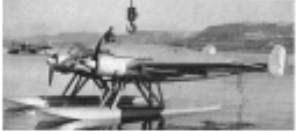
\includegraphics[width=30mm]{stato}};
    \node (a1) [left=25mm of a2] {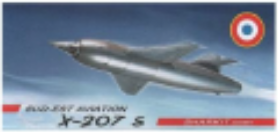
\includegraphics[width=30mm]{hydravion}};
    \node (a3) [right=25mm of a2] {
\includegraphics[width=30mm]{sudaviation}};

    \node (c1) [below=25mm of b1] {
\includegraphics[width=30mm]{snias}};
    \node (c2) [right=25mm of c1] {
\includegraphics[width=30mm]{aerospatiale}};
    \node (c3) [right=25mm of c2] {
\includegraphics[width=30mm]{eurocopter}};

    \node (d3) [below=5mm of c3, my text] {1992: La division ``hélicoptère'' de l'entreprise Aerospatiale s'unit avec l'hélicoptériste allemand, MBB, pour donner naissance à Eurocopter.\\1998: Eurocopter devient Eurocopter EADS company en fusionnant avec le groupe espagnol CASA.};
    \node (d2) [left=5mm of d3, my text] {1984: la SNIAS devient AEROSPATIALE. Son activité est concentrée dans les domaines de l'aéronautique, de l'espace, ainsi que de l'étude et la production d'avions et d'hélicoptères};
    \node (d1) [left=5mm of d2, my text] {1970: SUD-AVIATION, NORD-AVIATION, SEREB fusionnent et donnent naissance à la SNIAS (Société Nationale industrielle aérospatiale).};

    \node (e) [below=25mm of d2] {
\includegraphics[width=120mm]{airbushelicopters}};

    \node (f) [below=5mm of e, my text] {2014: le groupe tourne une page de son histoire et se renomme Airbus Helicopters};

    \foreach \i/\j in {a1/a2, a2/a3, c1/c2, c2/c3}
    \path [my arrow] (\i) -- (\j);

    \path [my arrow] (a3) -| ($(b3.south east) + (5mm,0)$) |- ($(b2.south -| b3)!1/2!(c2.north -| b3) + (0,5mm)$) -| (c1);
    \path [my arrow] (c3) -| ($(d3.south east) + (5mm,0)$) |- ($(d3.south -| d3)!1/2!(e.north -| d3) + (0,5mm)$) -| (e);

  \end{tikzpicture}

\end{document}